% !TeX spellcheck = en_US
\section{Workspace management}\label{section:workspace}

In this chapter we will describe all features of workspace panel.

Workspace panel displays all files and directories(items) from workspace directory. Items are displayed in hierarchical structure representing hierarchy in file system. It also allows to do some basic file management. Thanks to this features, user doesn't have to exit program when he want to manage files. Path to workspace can be configured in user settings. See \hyperref[section:user-settings]{User settings section}.

\begin{figure*}[!ht] 
	\centering
	\makebox[\textwidth]{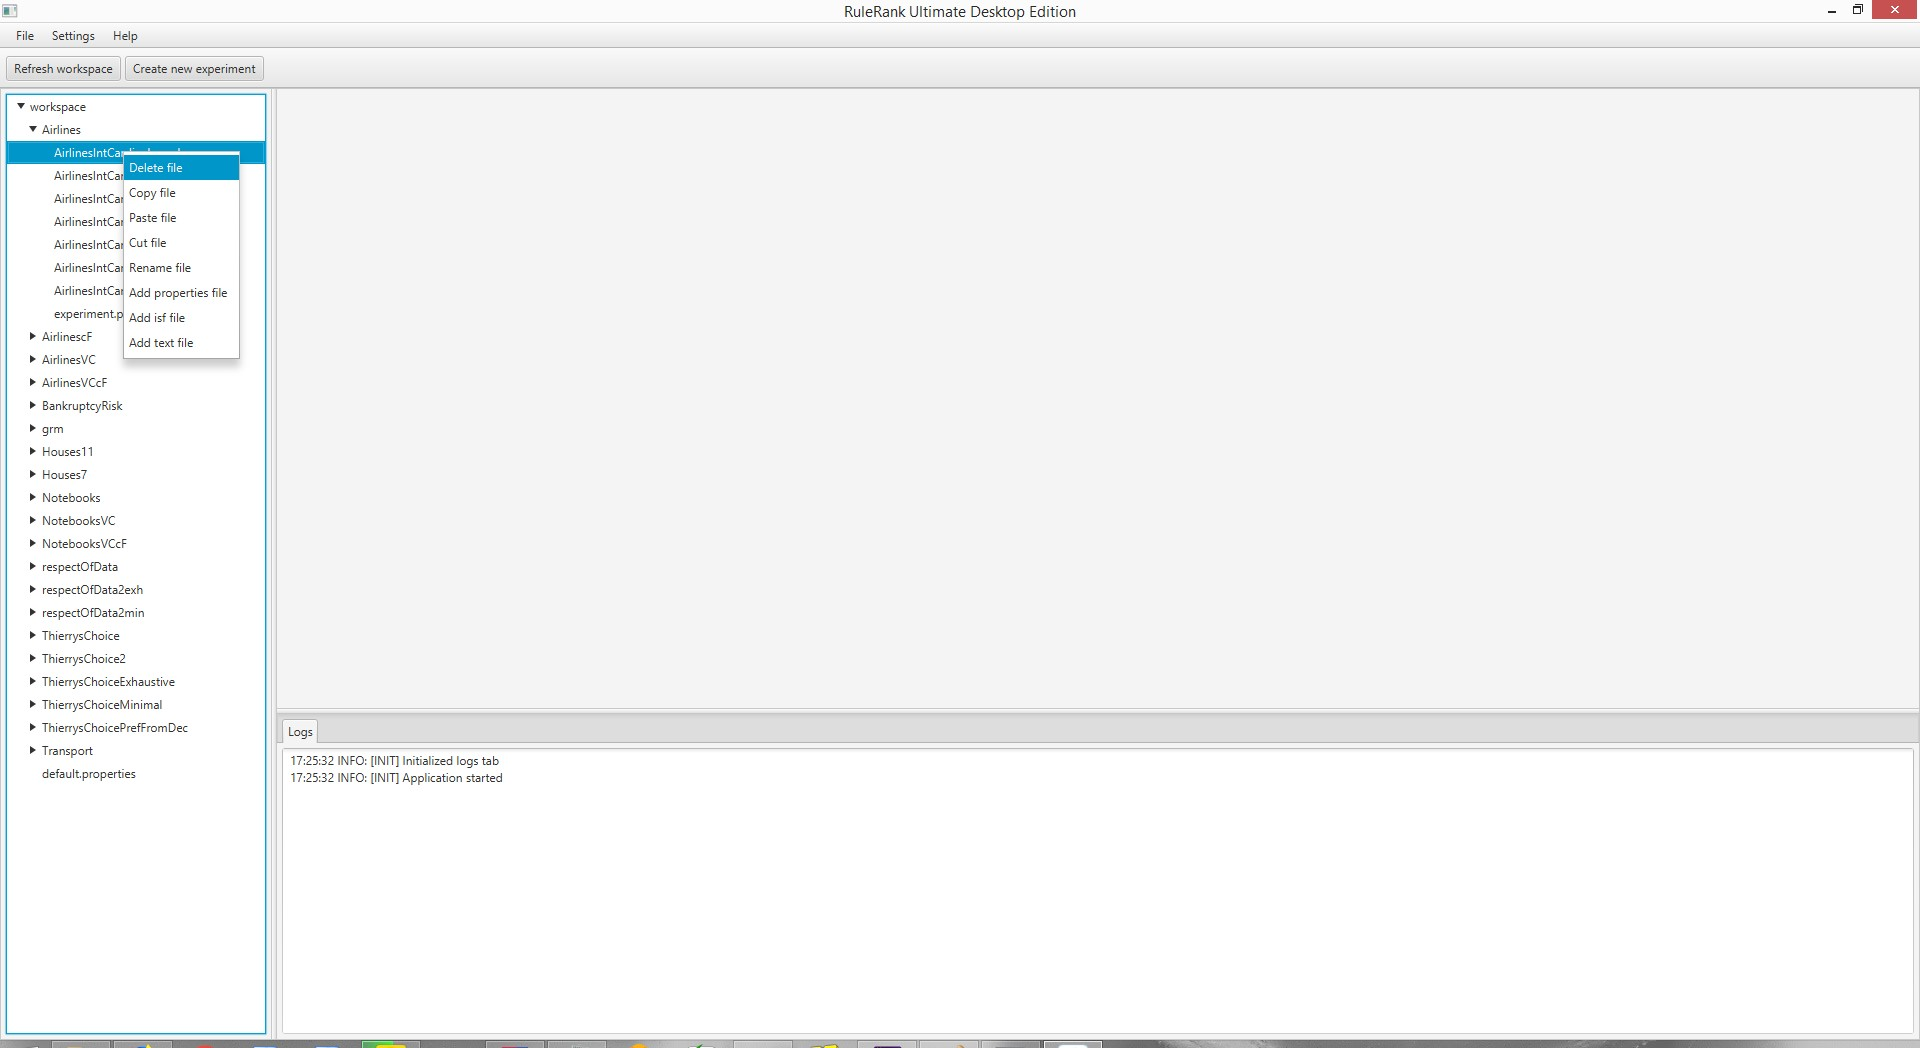
\includegraphics[width=.35\paperwidth]{workspace}}
	\caption{Application workspace from left panel}
\end{figure*}

Most of workspace functionality is provided by context menu, with is accessible by right clicking on workspace item(file or directory). If directory contains files or other directories, it will have arrow on left side indicating, that item can be expanded/hided. Buttons on toolbar are also used for workspace management. They contain actions with are not related with specific item. File can be opened by double clicking on it.

Some actions support keyboard shortcuts. To perform action by shortcut, you have to select item and press specific combination of keyboard buttons described below:
\begin{itemize}
	\item \textbf{Ctrl + C} - copies selected file to user clipboard. Copying directories is not supported yet.
	\item \textbf{Ctrl + V} - paste file to selected directory. If file was selected, file from clipboard will be copied to same directory as selected file.
	\item \textbf{Ctrl + X} - cuts file to user clipboard. If you paste file, old file will be removed.
	\item \textbf{Ctrl + R} - open dialog to rename file.
\end{itemize}


Toolbar currently supports two actions:

\begin{itemize}
	\item \textbf{Refresh workspace} - it refresh first level of workspace tree. If some directories were expanded deeper, they will be hided.
	\item \textbf{Create new experiment} - it allows to create new experiment with example isf table and experiment properties file. It will open dialog with shows workspace. You should create new directory there or choose existing directory.
\end{itemize}


It is recommended to create separate directory for each experiment. Learning or test data table(isf files) can be stored in commonly shared folders. Each directory should contain only one experiment properties file. This file is needed for other files to extract information about experiment. Also it is recommended to store results files in same directory as experiment properties file.\\

Below is supported file type list:
\begin{itemize}
	\item \textbf{.properties} - contains experiment properties with is used to configure experiment. See \hyperref[section:properties]{Experiment properties section}.
	\item \textbf{.isf} - contains tabular data with can be editable or read only depending on data type. Here you can configure learning or test data for experiment. You can also view partial pairwise comparison table generated by experiment.
	See \hyperref[section:isf-table]{Isf table edition section} and  \hyperref[sub:pct-isf]{Partial PCT section}.
	\item \textbf{.apx} - contains approximations of S and Sc relations in Pairwise Comparison Table, for now it is only displayed as text.
	See \hyperref[sub:pct-apx]{Partial PCT section}.
	\item \textbf{.rules} - contains generated rules and rules statistics.
	See \hyperref[section:rules]{Rules section}.
	\item \textbf{.graph} - contains preference graph visualization.
	See \hyperref[section:graph]{Graph visualization section}.
	\item \textbf{.ranking} - contains result ranking for experiment.
	See \hyperref[section:ranking]{Ranking window section}.
	\item \textbf{.txt} - it can be used to store some notes or to show experiment report
\end{itemize}

All other file types are not supported. Not supported files are treated as non editable text files.

\vfill\newpage